\section{Qu'est ce que le Cloud Computing ?}

Le Cloud Computing ( ou ``Informatique dans les Nuages" en français) est un secteur de l'informatique en plein essor depuis quelques années.
Un de ses concepts fondateurs est la mise à disposition de technologies et services à la demande : \textit{``as a service"}.

La vision est d'offrir aux utilisateurs un service à la demande où celui ci ne paie que sa consommation (une analogie avec le service  d'eau, d'électricité, de gaz peut être établie en France contrairement à certaines villes comme Moscou où l'on paie un forfait à l'année pour le gaz en illimité).

Cette technologie est actuellement en plein essor. De nombreux acteurs misent sur cette nouvelle manière d'envisager l'informatique. Parmi lesquels nous retrouvons Google, Amazon, Microsoft, IBM, SalesForce, DropBox, Apple, ... Des technologies à la fois orientés grand public et entreprises sont développés. Je citerai par exemple le Google Drive et Google Apps qui sont en fonction chez Valeo.\\
De plus en plus de domaines sont à présent concernés : \emph{Emails, Traitement de Texte, Stockage de Données, Jeux ...}

Le ``Cloud" se base sur une faculté native à s'adapter de manière élastique aux besoins des utilisateurs. À fournir des services en temps réel ou en ponctuel, à forte ou faible capacité (en terme de débit de connexion et de capacité de calcul). Ce sont tous ces facteurs qui font du ``Cloud" une valeur montante de l'informatique.

 \begin{figure}[H]
    \centering
    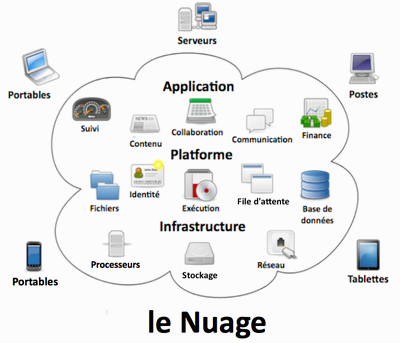
\includegraphics[height=9cm]{cloud.png}
	\caption{Représentation du Cloud}\label{image.cloud} 
\end{figure}